% --- [ Decompilation Phases ] -------------------------------------------------

\subsection{Decompilation Phases}
\label{sec:lit_review_decompilation_phases}

A core principle utilized in decompilers is the separation of concern through the use of abstractions, and extensive work involves translating into and breaking out of various abstraction layers. In general, a decompiler is composed of distinct phases which parses, analyses or transforms the input. These phases are conceptually grouped into three modules to separate concerns regarding source machine language and target programming language. Firstly, the front-end module parses executable files and translates their platform dependent assembly into a platform independent intermediate representation (IR). Secondly, the middle-end module performs a set of decompilation passes to lift the IR, from a low-level to a high-level representation, by reconstructing high-level control structures and expressions. Lastly, the back-end module translates the high-level IR to a specific target programming language \cite{reverse_comp}. Figure \ref{fig:modules_overview} gives an overview of the decompilation modules and visualizes their relationship.

\begin{figure}[htbp]
	\begin{center}
		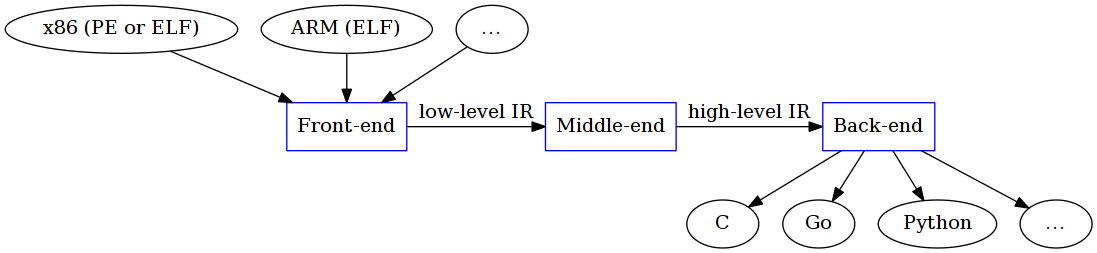
\includegraphics[width=\textwidth]{inc/modules_overview.png}
		\caption{Firstly, the front-end module accepts several executable file formats (PE, ELF, …) as input and translates their platform dependent assembly (x86, ARM, …) to a low-level IR. Secondly, the middle-end module then lifts the low-level IR to a high-level IR through a set of decompilation passes. Lastly, the backend-module translates the high-level IR into one of several target programming languages (C, Go, Python, …).}
		\label{fig:modules_overview}
	\end{center}
\end{figure}

The remainder of this section describes the distinct decompilation phases, most of which have been outlined by Cristina Cifuentes in her influential paper \textit{``Reverse Compilation Techniques''} \cite{reverse_comp}.

% --- [ Subsubsections ] -------------------------------------------------------

% ~~~ [ Binary Analysis ] ~~~~~~~~~~~~~~~~~~~~~~~~~~~~~~~~~~~~~~~~~~~~~~~~~~~~~~

\subsubsection{Binary Analysis}
\label{sec:lit_review_binary_analysis}

As demonstrated in section \ref{sec:lit_review_the_anatomy_of_an_executable}, parsing even a simple \textit{``hello world''} executable requires extensive knowledge of its binary file format (in this case ELF). The binary analysis phase is responsible for parsing input files of various binary file formats, such as PE and ELF, and present their content in a uniform manner which preserves the relations between file contents, virtual addresses and access permissions. Later stages of the decompilation pipeline builds upon this abstraction to access the file contents of each segment or section without worrying about the details of the underlying file format. Information about external symbols, metadata and the computer architecture of the assembly may also be provided by this abstraction.

% ~~~ [ Disassembly ] ~~~~~~~~~~~~~~~~~~~~~~~~~~~~~~~~~~~~~~~~~~~~~~~~~~~~~~~~~~

\subsubsection{Disassembly}

The disassembly phase (referred to as the \textit{syntactic analysis phase} by C. Cifuentes) is responsible for decoding the raw machine instructions of the executable segments into assembly. The computer architecture dictates how the assembly instructions and their associated operands are encoded. Generally CISC architectures (e.g. x86) use variable length instruction encoding (e.g. instructions occupy between 1 and 17 bytes in x86) and allow memory addressing modes for most instructions (e.g. arithmetic instructions may refer to memory locations in x86) \cite{x86_manual}. In contract, RISC architectures (e.g. ARM) generally use fixed-length instruction encoding (e.g. instructions always occupy 4 bytes in AArch64) and only allow memory access through load-store instructions (e.g. arithmetic instructions may only refer to registers or immediate values in ARM) \cite{arm_manual}.

One of the main problems of the disassembly phase is how to separate code from data. In the Von Neumann architecture the same memory unit may contain both code and data. Furthermore, the data stored in a given memory location may be interpreted as code by one part of the program, and as data by another part. In contrast, the Harvard architecture uses separate memory units for code and data \cite{von_neumann_vs_harvard}. Since the use of the Von Neumann architecture is wide spread, solving this problem is fundamental for successful disassemblers.

% TODO: Add switch tables example.

A solution to the problem of separating code from data is to use recursive descent instead of linear descent when parsing assembly instructions.

% TODO: Add description of recursive descent and linear descent.

\begin{figure}[htbp]
	\centering
	\begin{subfigure}[t]{0.49\textwidth}
		\lstinputlisting[language=nasm, style=nasm, tabsize=2]{inc/hello/hello_linear.asm}
		\caption{Disassembly from \texttt{objdump} and \texttt{ndisasm}\protect\footnotemark.}
	\end{subfigure}
	\qquad
	\begin{subfigure}[t]{0.35\textwidth}
		\lstinputlisting[language=nasm, style=nasm, tabsize=2]{inc/hello/hello_recursive.asm}
		\caption{Disassembly from IDA Pro.}
	\end{subfigure}
	\caption{The disassembly produced by a linear descent parser (left) and a recursive descent parser (right) when analyzing a simple \textit{``hello world''} program that stores the \texttt{hello} string in the executable segment.}
\end{figure}
\footnotetext{The Netwide Disassembler: \url{http://www.nasm.us/doc/nasmdoca.html}}

One problem faced by both linear descent and recursive descent disassemblers is the need for a starting point. In practise, exported entry point symbols (e.g. \texttt{main}, \texttt{start}, \texttt{DLLMain}, …) works well.

% TODO: Verify that it is called symbolic execution/symbolic execution engine.

Another problem for recursive descent disassemblers is indirect branches (e.g. jump to the address stored in a register). In the case of indirect branches, it is impossible to know the branch target by only looking at the individual instructions. One solution is to use symbolic execution, which emulates the processor and executes instructions to give information about the value stored in registers. With this method the target of indirect jumps may be calculated. There are problems to consider when designing a symbolic execution engine, for instance the impact of cached memory access. See figure \ref{foo} for an example of where cache details matter for the execution flow.

% TODO: Add example where the cache impacts execution flow (pipeline pre-schedules). *addr = 5; jmp addr

% Problems:
% * self-modifying code
% * Architecture-dependent Restrictions
%    Cannot be determined by step-by-step debugging; as the prefetch pipeline
%    would behave differently.
%       mov ax, 0x9090
%       mov [jmpDef], ax
%    jmpDef:
%       jmp codeExecuted
%    codeNotExecuted:
%       foo
%    codeExecuted:
%       bar

Another issue is the use of callbacks, which is common in GUI applications.
% TODO: Solution? Run program and use breakpoints?

There exists several anti-disassembly techniques which are commonly used by malware. One such technique exploits the fact that recursive descent parsers follow both the true and the false branch of conditional branch instructions, as demonstrated in figure \ref{fig:anti-disassembly}.

The recursive descent parser cannot parse both the false and the true-branch of the conditional branch instruction at line 3, because the true branch targets the middle of a \texttt{jmp} instruction.

The conditional branch instruction at line 3 always takes the true branch, which points to the middle of the \texttt{jmp} instruction decoded when parsing the false branch. The recursive descent parser cannot disassembly both branches and is forced to choose one of them, in this case the \texttt{fake} branch.

The recursive descent parser fails by using a conditional branch instruction (\texttt{jz}) which always takes the true-branches \texttt{fake+1} which is in the middle of an instruction.

\begin{figure}[htbp]
	\centering
	\begin{subfigure}[t]{0.59\textwidth}
		\lstinputlisting[language=nasm, style=nasm, tabsize=2]{inc/hello/anti_orig.asm}
		\caption{Original assembly.}
	\end{subfigure}
	\qquad
	\begin{subfigure}[t]{0.34\textwidth}
		\lstinputlisting[language=nasm, style=nasm, tabsize=2]{inc/hello/anti_fail.asm}
		\caption{Disassembly from IDA Pro.}
	\end{subfigure}
	\caption{The original assembly (left) contains an anti-disassembly trick which causes the recursive descent parser to fail (right).}
	\label{fig:anti-disassembly}
\end{figure}

The anti-disassembly technique presented in figure \ref{fig:anti-disassembly} may be mitigated using symbolic execution, which could verify that the conditional jump always takes the true branch and therefore allow the instruction to be replaced with an unconditional jump to the target of the true branch. This quickly becomes a game of cat-and-mouse, as the anti-disassembly techniques could be extended to rely on network activity, file contents, or other external sources which would render the symbolic exeuction useless.

To conclude, the disassembly phase deals with non-trivial problems, some of which are difficult to automate. Advanced disassemblers therefore provide interactive capabilities and rely on human intuition to solve ambiguities and direct the disassembler out of corner cases. See section \ref{sec:related_work_hex-rays_decompiler} for further details on such disassemblers.

% TODO: Introduce the various approaches and highlight their individual
% strengths and weaknesses.
%
% NAIVE APPROACH: linear descent disassemblers.
% PROBLEM: Highlight problems with linear descent disassemblers.
%    - rodata (e.g. "hello world") and jump tables in code.
%
% SOLUTION: recursive descent disassemblers.
% PROBLEM: Highlight problems with recursive descent disassemblers.
%    - Distinguish between code and data (e.g. find entry points of functions).
%      Not add functions are directly referred to (e.g. callback functions which
%      are commonly used by GUI applications).
%    - Easy to fool.
%       xor eax, eax
%       cmp eax, 0
%       jz foo+1 ; Cannot disassembly both foo and foo+1.
% foo:
%       add eax, 3
%
% SOLUTION: symbolic execution engines.
% PROBLEM: security, performance, ...?

% ~~~ [ Semantic Analysis ] ~~~~~~~~~~~~~~~~~~~~~~~~~~~~~~~~~~~~~~~~~~~~~~~~~~~~

\subsubsection{Semantic Analysis}

foo

% TODO: Ideoms
%    - 64-bit binops
%    - xor eax, eax ; eax = 0

% ~~~ [ Intermediate Code Generation ] ~~~~~~~~~~~~~~~~~~~~~~~~~~~~~~~~~~~~~~~~~

\subsubsection{Intermediate Code Generation}
\label{sec:lit_review_intermediate_code_generation}

% TODO: <note> remove?
% "Most compilers translate the source program first to some form of intermediate representation and convert from there into machine code. The intermediate representation is a machine- and language-independent version of the original source code. Although converting the code twice introduces another step, use of an intermediate representation provides advantages in increased abstraction, cleaner separation between the front and back ends, and adds possibilities for re-targeting/cross-compilation. Intermediate representations also lend themselves to supporting advanced compiler optimizations and most optimization is done on this form of the code."

% * Subroutines included by the compiler and linker; to which phase does this belong?
%    Bloat.

foo

% ~~~ [ Control Flow Graph Generation ] ~~~~~~~~~~~~~~~~~~~~~~~~~~~~~~~~~~~~~~~~

\subsubsection{Control Flow Graph Generation}

foo

% ~~~ [ Data Flow Analysis ] ~~~~~~~~~~~~~~~~~~~~~~~~~~~~~~~~~~~~~~~~~~~~~~~~~~~

\subsubsection{Data Flow Analysis}

foo

\cite{type_based_decomp}

% ~~~ [ Control Flow Analysis ] ~~~~~~~~~~~~~~~~~~~~~~~~~~~~~~~~~~~~~~~~~~~~~~~~

\subsubsection{Control Flow Analysis}

Control-Flow Graph (CFG)

foo

% TODO: Add notes about irriducible graphs; may be solved using node splitting.
% * functional (semantics?) vs. forensic equivalence.

% ~~~ [ Code Generation ] ~~~~~~~~~~~~~~~~~~~~~~~~~~~~~~~~~~~~~~~~~~~~~~~~~~~~~~

\subsubsection{Code Generation}

foo

